\begin{center}
\textbf{Modeling the Construction and Evolution of Distributed Volcanic Fields on Earth and Mars}
\end{center}

\section*{Introduction}
Magmatism is a dominant process on Earth and Mars that has significantly modified and evolved the lithospheres of each planet by delivering magma to shallow depths and to the surface, forming volcanoes. Two common modes of volcanism are present on both Earth and Mars: central-vent dominated volcanism that creates large edifices from concentrating magma in chambers before eruptions and distributed volcanism that creates many smaller edifices on the surface through the independent ascent of individual magmatic dikes. In regions of distributed volcanism, clusters of volcanoes develop over thousands to millions of years \citep{valentine2000basaltic}. This dissertation explores the geology of distributed volcanism on Earth and Mars from shallow depths ($\sim$1~km) to the surface. 

Each edifice in a volcanic field, often a scoria cone, lava dome, or maar diatreme, is most often created from the arrival of a single magmatic dike to the surface during a single eruptive phase that lasts from weeks to decades. The term ``monogenetic volcano,'' used to describe scoria cones, small shield volcanoes, and maar volcanoes, comes from this concept of single eruptions forming small volcanoes \citep{greeley1977basaltic}, though individual scoria cones sometimes exhibit recurring volcanic activity over tens to hundreds of years \citep{hill1998cerro}. Distributed-style volcano clusters, forming from dikes ascending through lithosphere from a magma source hundreds to many thousands of square kilometers in extent, are reflections of properties of both their source region and the lithospheric filter \citep{settle1979structure}.

People have lived within volcanic fields since pre-historic times and their livelihoods have been affected when eruptions occur, usually with little to no warning \citep{elson2007living}. Recently, spacecraft have been sent to other planets, revealing the existence of distributed-style volcanism on Mars \citep{carr1977some} and Venus \citep{head1992venus}. On these neighboring planets, tens to tens of thousands of distributed volcanic vents form patchworks of shield volcanoes \citep{richardson2013volcanic,miller2012shield}. 

%\begin{wrapfigure}{l}{0.65\textwidth}
\begin{figure}[hb!]
\centering
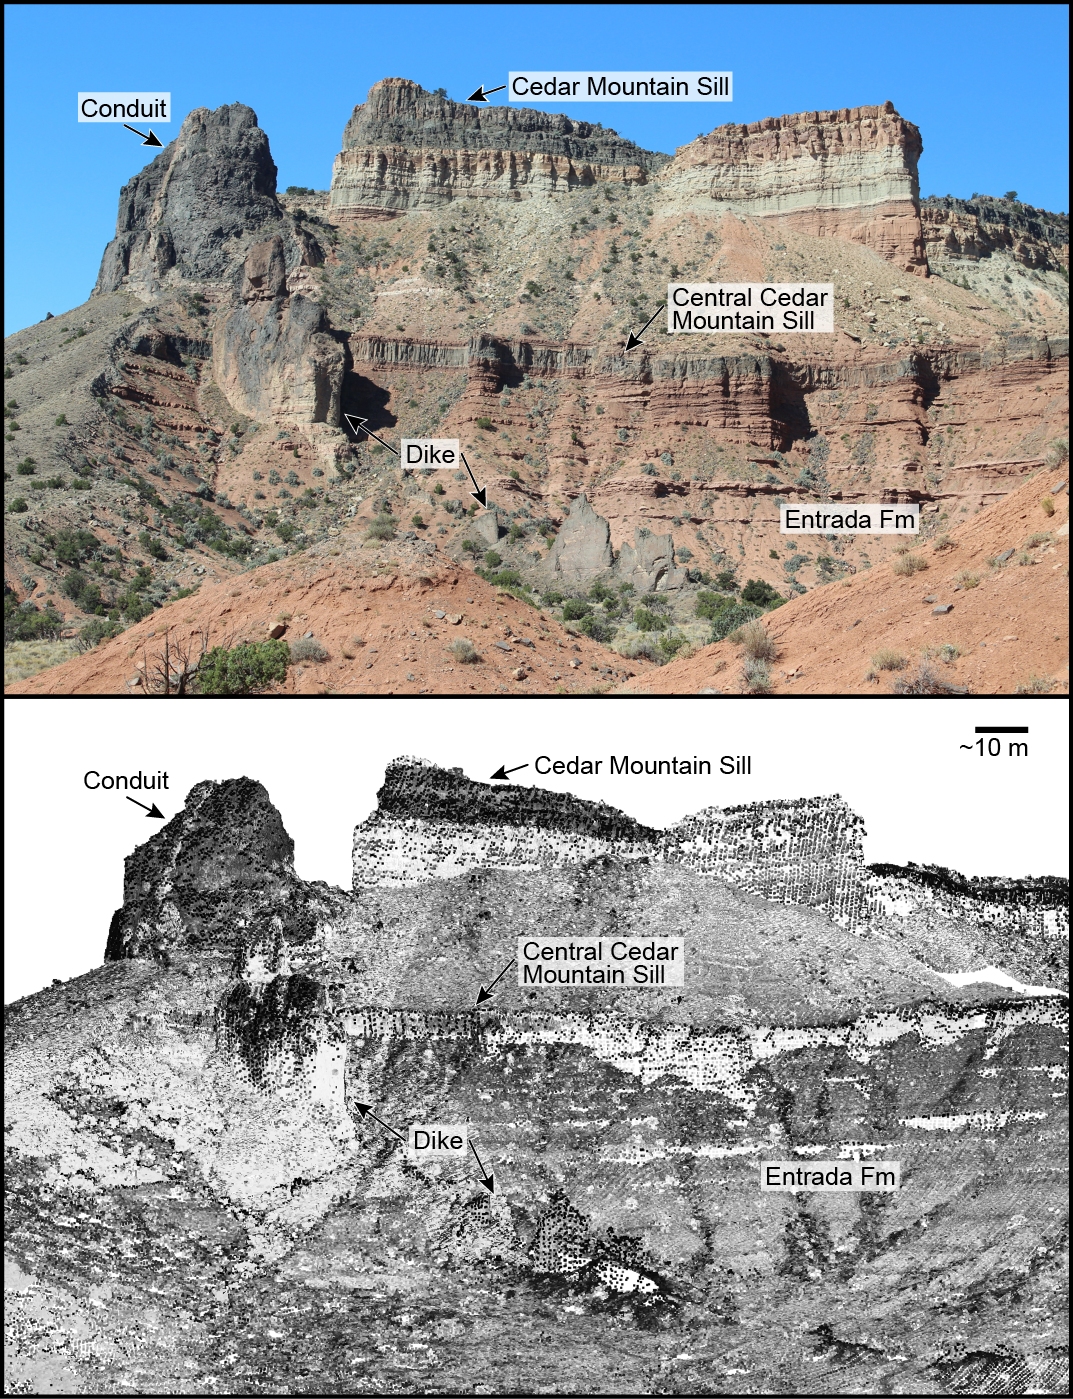
\includegraphics[width=0.6\textwidth]{figures/chapter-sills/SFig2-photo_pcloud}
\caption{Photograph (top) and a combined terrestrial/aerial lidar point cloud (bottom) of the east face of Cedar Mountain (Central Utah, USA) two sills and a dike which cross-cuts the lower sill. Sills are separated by dozens of meters by sedimentary rock. Near-Infrared intensity differentiates between igneous and sedimentary rocks in the point cloud.}
\label{fig_photo-pcloud}
\end{figure}
%\end{wrapfigure}

This dissertation addresses five different aspects of distributed volcanic fields. The first chapter focuses on the role of the magma plumbing system in the evolution of volcanic fields. I use lidar datasets (Figure \ref{fig_photo-pcloud}) to model magmatic sills in the San Rafael Swell, Utah \citep{richardson2015sills}. Second, a lava flow simulator is validated and used to model a recent lava flow. This simulator has modeled the 2012-3 Tolbachik lava flow in Kamchatka, Russia, using flow characteristics derived from TanDEM-X InSAR data \citep{kubanek2015lava}. Third, two chapters focus on volcano clusters on Mars, characterizing the long-term evolution of two fields. The first of these (Chapter 3) studies the Syria Planum region \citep{richardson2013volcanic}. The second (Chapter 4) focuses on Arsia Mons \citep{richardson2015recurrence}. The final chapter models and compares the spatial density of volcanic vents in clusters on Earth, Mars, and Venus \citep{richardson2012comparison}.


\section{Role of sills in the development of volcanic fields}

In Chapter 1, terrestrial and airborne lidar data are used to map volcanic features in the San Rafael Swell (Utah, USA) (Figure \ref{fig_photo-pcloud}). The San Rafael Volcanic Field is a Pliocene-aged volcanic field that has been eroded to a depth of $<$1~km exposing the igneous intrusion network. Analysis of the combined lidar datasets enables modeling of the geometries of seven magmatic sills. The total volume of these sills is $>$0.4~km$^3$, with each sill containing 10$^{-4}$-10$^{-1}$ km$^3$ of igneous rock. Mapped sill volumes account for $>$92\% of intrusive material within the 25~km$^3$ block that geometrically bounds the study area, with the rest of the material being stored in dikes and volcano conduits.

Sills in the San Rafael likely played a significant role in modifying eruption dynamics. At least one sill formed cotemporally with an eruption. Depending on the conduit diameter and the adjacent co-magmatic sill height, gas would have been entrained in either the conduit or the sill, modulating eruption explosivity.


\section{A fast code for probabilistically modeling lava flows}

In Chapter 2, a cellular auto\-mata \citep{wolfram1984cellular} lava flow simulator is developed following the algorithm of \citet{connor2012probabilistic}. The simulator, named MOLASSES, has been developed in C with a modular framework, which enables users to quickly change relatively few lines of code to modify the flow behavior.


MOLASSES is used to probabilistically model the 2012-3 Tolbachik lava flow (Kamchatka, Russia), using flow characteristics measured with TanDEM-X InSAR results. Figure \ref{fig_MC_map} illustrates the outcome of a Monte Carlo simulation over a Shuttle Radar Topography Mission (SRTM) elevation model. By incorporating uncertainties inherent to each input parameter (e.g. elevation, flow thickness uncertainty) into the MOLASSES simulations, a model of how likely an area is to be inundated is produced. This probability map correlates well with the true inundation of the Tolbachik flow and may be used as a future tool for forecasting lava flow hazard during volcanic crises.

\begin{figure}[hb!]
%\begin{wrapfigure}{r}{0.6\textwidth}
	\centering
	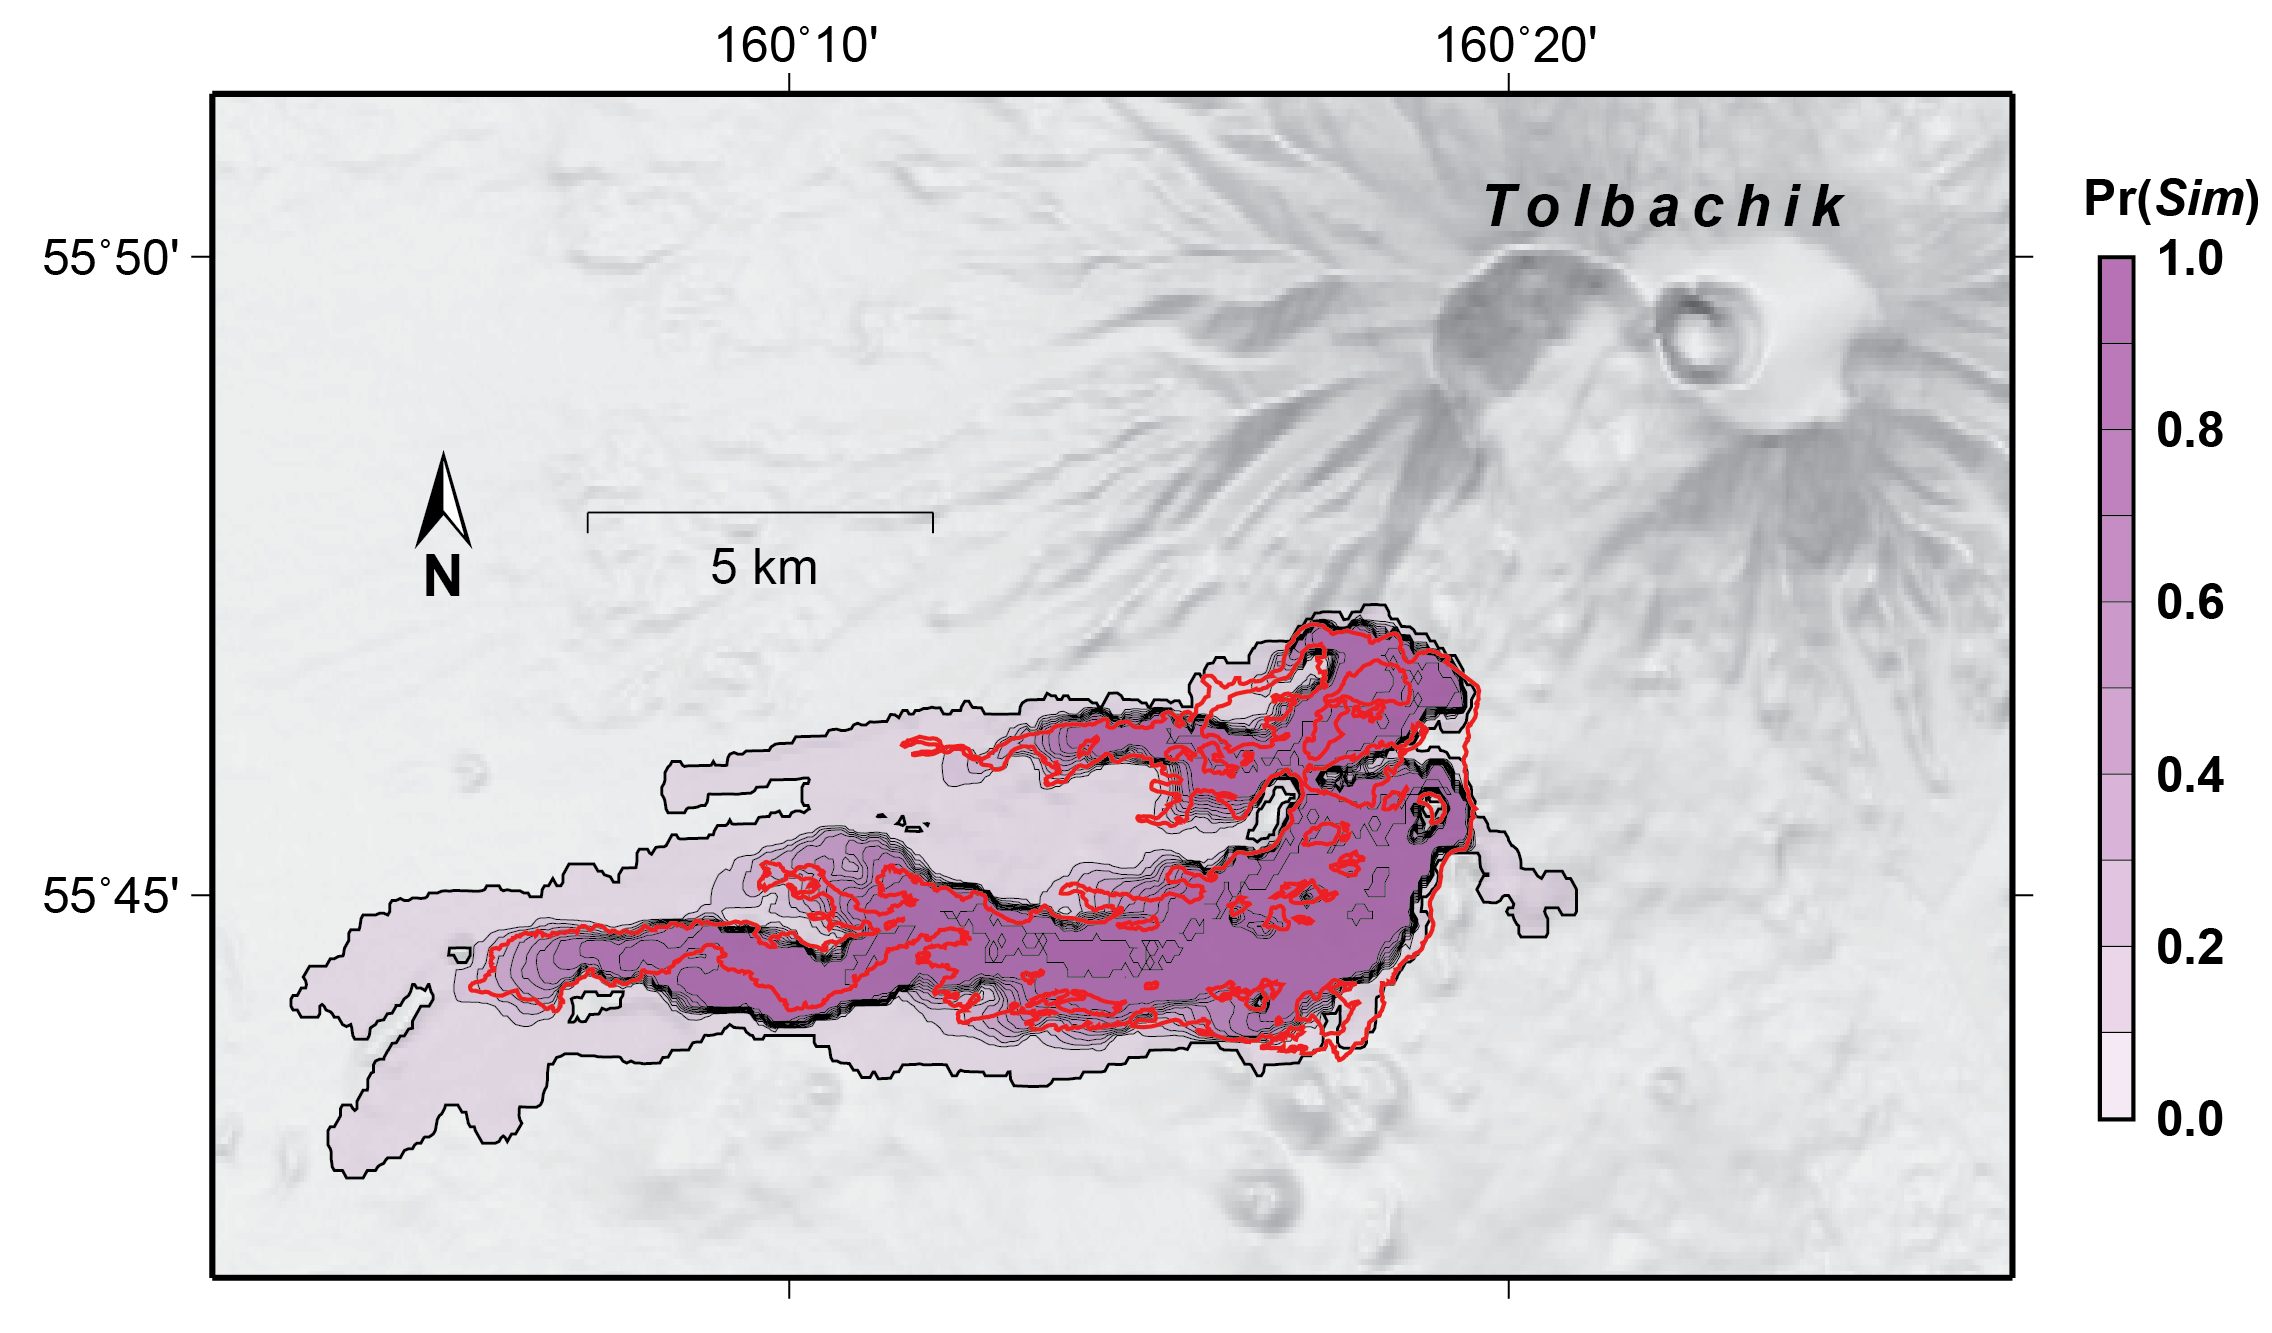
\includegraphics[width=0.65\textwidth]{figures/chapter-molasses/MC_probmap_300dpi}
	\caption{Cumulative distribution of 100,000 simulated lava flows over SRTM topography with 3~m elevation uncertainty. The red outline is the mapped flow extent of the 2012-3 Tolbachik flow. Darker purple areas represent more simulation hits (i.e. higher $\text{Pr}(Simulation)$).}
	\label{fig_MC_map}
%\end{wrapfigure}
\end{figure}

\section{The volcanic history of Syria Planum, Mars}

\begin{figure}[h]
	\centering
	\includegraphics[width=0.7\linewidth,clip,trim=0.8cm 5cm 0.9cm 0.1cm]{figures/chapter-syria_planum/fig1-eps-converted-to.pdf}
	\caption{Geologic Map of Syria Planum, Mars, over a shaded relief basemap. Volcanism in this field evolved from central-vent dominated lavas (unit Hsm), to coalesced small shields (unit Hssf), to a northern coalesced unit (Hnsf). Point features are volcanic vents (black, vent is visible; white, likely vent; star, Syria Mons) and graben are shown as thin black lines.}
	\label{fig-geomap}
\end{figure}

In Chapter 3, a field of distributed shield volcanoes in the Syria Planum region of Mars is mapped to determine abundance, distribution, and alignments of vents (Figure \ref{fig-geomap}). Nearest neighbor and two--point azimuth analyses are conducted, using mapped volcanic vent locations, to assess the spacing and orientations between vents across the study area. Two vent fields are identified as unique volcanic units along with the previously identified Syria Mons volcano. Superposition relationships and crater counts indicate that these three volcanic episodes span $\sim$900 Ma, beginning in the early Hesperian Period and ending in the Early Amazonian Period (3.5-2.6~Ga). No clear hiatus in eruptive activity is identified between these events, as crater age-dating error bars of each unit abut the modeled ages of other units. However, activity migrates from eruptions at Syria Mons, to regionally distributed eruptions that form the bulk of the Syria Planum plains, to dispersed eruptions in Syria's northwest. 


Nearest neighbor analyses suggest a non--random distribution among the entire population of volcanoes comprising Syria Planum, which is interpreted to result from the interaction of independent magma bodies ascending through the crust during different stress regimes throughout the region's eruptive history. Two--point azimuth results identify three orientations of enhanced alignments, which match well with radial extensions of three major tectonic centers to the south, east, and northwest of the study area. 

As such, Syria Planum volcanism evolved from a central vent volcano to dispersed shield field development over several hundred million years, an extremely long timeframe compared with Earth volcanism, during which the independent magma bodies related to each small volcano interacted to some extent with one or more of at least three buried tectonic patterns in the older crust.


\section{Waning volcanism on Arsia Mons, Mars}
In Chapter 4, the recurrence rate of a volcanic field in the 110~km caldera of Arsia Mons, Mars, is modeled by combining stratigraphy and crater retention rate age modeling. In this caldera, 29 volcanic vents have been mapped and each have long lava flows extending several to tens of kilometers downhill. Vents in this caldera are comparatively young ($\sim$130~Ma on average), since no craters in the floor are larger than 1~km in diameter. The age of each vent can be modeled with crater counts, but the age uncertainty associated with this method can be larger than the total age of the field. To better quantify crater age model uncertainty, stratigraphic information has been added, since each lava flow embays or is embayed by at least one adjacent flow.

	\begin{figure}[h!]
		\centering
		\begin{gnuplot}[terminal=latex, terminaloptions=rotate]
			unset key
			set size 1,0.9
			set format xy "$%g$"
			set xlabel "Time before present, Ma" rotate by 90
			set ylabel "Volume Flux\n\n10 m flows (km$^3$ Myr$^{-1}$)"
			set y2label "Volume Flux\n\n80 m flows (km$^3$ Myr$^{-1}$)"
			set xrange [350:0]
			set yrange [0:4.5]
			set y2range [0:36]
			set ytics 1
			set y2tics 8
			set xtics 100
			plot "data/Arsia_Mons_10m_THICK_CORRECTED_time_predict_crater_neighbor.dat" using 1:2 with lines lt 4, "data/Arsia_Mons_10m_THICK_CORRECTED_time_predict_crater_neighbor.dat" using 1:4 with lines lt 4, "data/Arsia_Mons_10m_THICK_CORRECTED_time_predict_crater_neighbor.dat" using 1:3 with lines lt 5
		\end{gnuplot}
		\caption{Modeled volume flux for the latest effusive activity within Arsia Mons Caldera, assuming mapped units have an average thickness of 10~m (left axis) or 80~m (right axis). The median flux of the MC simulations is plotted with a 90\% confidence envelope. Volume flux is interpreted to remain relatively constant between 150-100~Ma (0.4~km$^3$~Myr$^{-1}$ assuming 10~m thick units or 3~km$^3$~Myr$^{-1}$ for 80~m thick units).}
		\label{fig_VERRMAREA}
	\end{figure}

An algorithm has been created to identify potential ages of each vent based on crater age models and stratigraphy. This algorithm, named the Volcanic Event Recurrence Rate Model (VERRM), is then used in a Monte Carlo fashion to create 100,000 possible vent age sets. The recurrence rate of volcanism with respect to time is calculated for each possible age set, and these rates are combined to calculate the median recurrence rate of all simulations. This method finds that, for the 29 volcanic vents, distributed volcanism likely began within the caldera around 200~Ma then peaked around 150~Ma, with an average production rate of 0.25~vents per Ma. Volcanism then waned until the final vents were produced 10-90~Ma.

By applying modeled volumes to each volcano, volume flux rate is also calculated. Depending on the estimated volume, volume flux might have reached a peak rate of 0.1-3 km$^3$~Myr$^{-1}$ by 150~Ma and sustained this rate until about 90~Ma, when the volume flux diminished greatly.

The onset of volcanism of the 29 vents in the caldera at $\sim$200~Ma can be related to volcanic ash that was emplaced before 200~Ma on the flanks of Arsia Mons. The close timing of evidence of large, explosive volcanism and the oldest of the distributed effusive volcanoes might indicate that around 200~Ma the style of volcanism at Arsia Mons transitioned from explosive to effusive. If this transition took place, then the waning of recurrence rate of volcanism since 150~Ma might be the termination of larger magmatic activity related to construction of the Arsia Mons edifice.

\section{Uses of kernel statistics on volcanic vents}


Chapter 5 compares the spatial intensity of volcanic vents (vents per unit area) for volcano clusters on the Earth, Mars, and Venus, revealing a fundamental difference between clusters on the three planets (Figure \ref{fig_ventdens}). On Earth, vents in volcano clusters are packed at 0.1 vents~km$^{-2}$. On Mars, vents in clusters are two orders of magnitude more dispersed, at 0.001 vents~km$^{-2}$. On Venus, clusters have an intermediate density of 0.01 vents~km$^{-2}$. This change in distribution scale is due to differences in the structure and composition of the planets' lithospheres, as well as the way broad regions of magma generation are created.


\begin{figure}[h!]
	\centering
	\begin{gnuplot}[terminal=latex, terminaloptions=rotate]
		unset key
		set size 1,0.9
		set key l
		set logscale xy 10
		set xlabel "Vent count in volcano cluster" rotate by 90
		set ylabel "2-$\sigma$ Cluster Size (km$^2$)"
		set xrange [20:12000]
		set yrange [500:4e6]
		set label "10 km$^2$ per vent" at first 1500, first 1e4 rotate by 23
		set label "100 km$^2$ per vent" at first 1500, first 1e5 rotate by 23
		set label "1000 km$^2$ per vent" at first 600, first 4e5 rotate by 23
		plot "data/ventdens_model.dat" using 1:2 with lines lt 4 notitle,\
		"data/ventdens_model.dat" using 1:3 with lines lt 4 notitle,\
		"data/ventdens_model.dat" using 1:4 with lines lt 4 notitle,\
		"data/ventdens_earth.dat" using 1:2 with points pt 6 title "  Earth Clusters",\
		"data/ventdens_venus.dat" using 1:2 with points pt 7 title "  Venus Clusters",\
		"data/ventdens_mars.dat" using 1:2 with points pt 3 title "  Mars Clusters"
	\end{gnuplot}
	\caption{Volcano cluster size plotted with respect to the number of vents in the cluster. Three contours are drawn as dotted lines to show cluster vent intensity at 10, 100, or 1000 vents per km$^2$.}
	\label{fig_ventdens}
\end{figure}


Spatial intensity is modeled with Kernel Density Estimation, a non-parametric statistical tool that models point density as a 2D density distribution by assigning probability density functions (PDFs) to a population of mappable points. Volcanic vent locations from several catalogs are used to compare cluster characteristics across the Solar System, including vent catalogs created and used in Chapters 1, 3, and 4.

\begin{wrapfigure}{r}{0.51\textwidth}
\centering
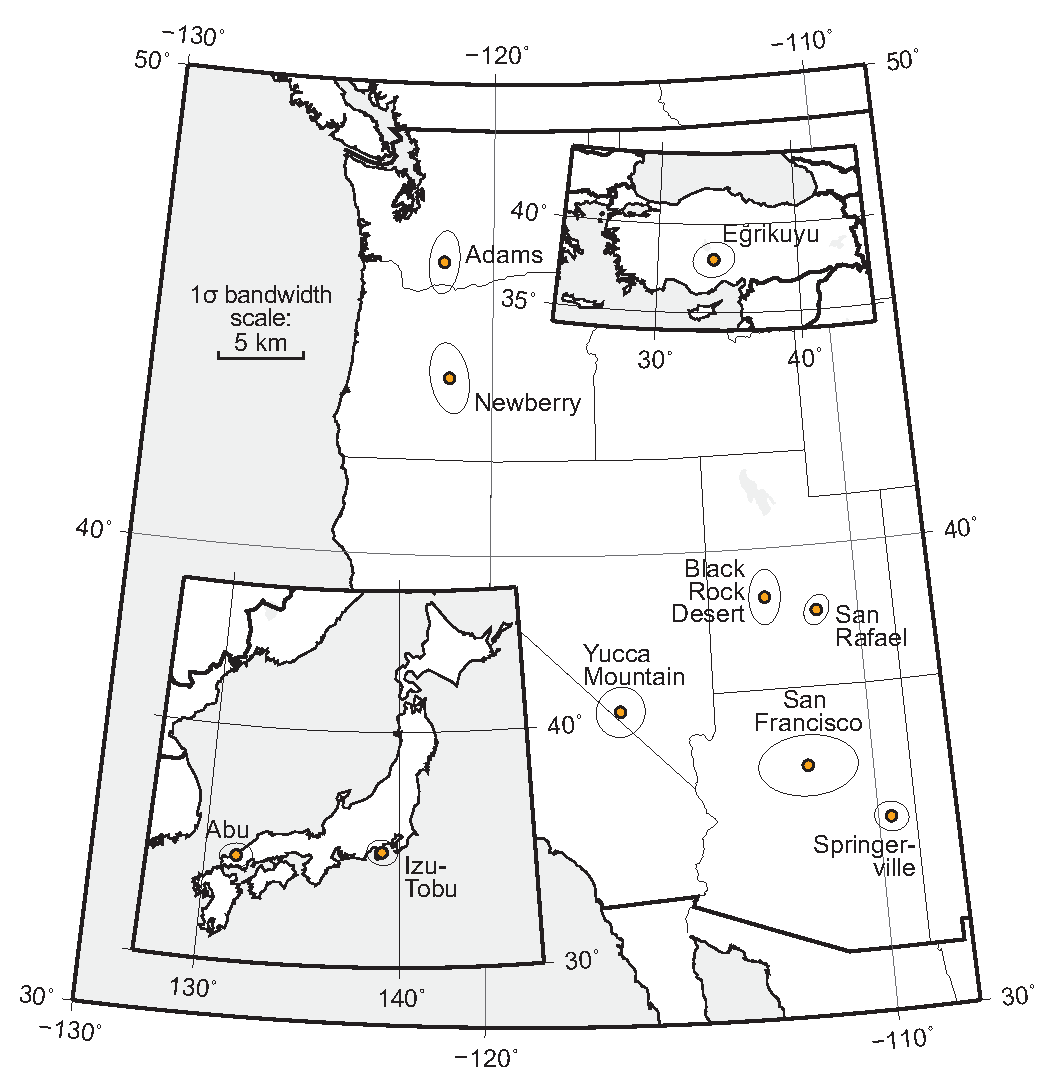
\includegraphics[width=0.5\textwidth]{figures/chapter-spatial_density/locators/earth_locator.eps}
\caption{Locations of selected volcano clusters on Earth. Kernel bandwidth ellipses (drawn over each location) are influenced by each field's magma source region and pre-existing features in the elastic lithosphere.}
\label{fig_earthlocator}
\end{wrapfigure}

The influences of the lithosphere and magma source region on dike formation and ascent are reflected in the distribution of volcanoes at the surface of a volcanic field. Here, Kernel Bandwidth (i.e. the width of the PDF used to model vent density for a volcano cluster) is used as a proxy of cluster elongation and orientation. Bandwidths, illustrated in Figure \ref{fig_earthlocator} are influenced by elongated magmatic source regions, source region migration, and pre-existing lithospheric features that enabled or inhibited magma focusing in different directions.

\clearpage
\section{Conclusion}

This dissertation provides a diverse set of views into the creation of distributed volcanic fields within the inner Solar System. It is found that volcanic features in fields have a spatial organization that is characteristic of the planet that they are on, with features on Earth clustering two orders of magnitude more densely than they might on Mars. This organization is governed by the location and productivity of a magma source region as well as the organization of pathways that magma exploits during ascent.

In the San Rafael Swell (Utah, USA), the pathways taken by magma in the Pliocene are now exposed, showing several sills, 52~km of dikes, and many volcanic conduits. Each intrusion in this field area was emplaced during a relatively short time period (likely $<$100 years), with long hiatuses between events. Some intrusions are identified to have been emplaced as part of one event, and it is seen that the creation of shallow sills during or immediately preceding a volcanic eruption will modulate eruption style.

In the Tharsis Volcanic Province of Mars, the long term evolution of two volcanic fields have been studied. Results from the Syria Planum volcanic field show that a single region on Mars can host volcanism for nearly 1~Gyr. Volcanoes within the caldera of Arsia Mons are used to model the magma flux over time for a volcanic field on Mars, showing that 0.4-3 km$^3$ per Myr of lava erupted to the surface of the caldera for roughly 50~Myr.

Modeling the emplacement of lava can now be performed using a modular code developed in this dissertation for hazards forecasting. MOLASSES has been validated using the 2012-3 Tolbachik lava flow in Kamchatka, Russia and accurately models the lava flow with a Predictive Value of $>$80\%. In the future this code will be used for hazards forecasting and as a geomorphology tool in modeling lava flow fields on Earth and Mars.

%%%%%%%%%%%%%%%%%%%%%%%%%%%%%%%%
%References
%%%%%%%%%%%%%%%%%%%%%%%%%%%%%%%%
\singlespacing
\setlength{\bibsep}{3pt}

%%%%%%%%%%%%%%%%%%%%%
%%References Section
\section{References}

\bibliography{dissertation_refs}
\bibliographystyle{apalike} 
